
\begin{center}
\Huge
Eksponentiel vækst og eksponentialfunktioner 2
\end{center}
\stepcounter{section}
Vi ser igen på et eksempel.
\begin{exa}\label{exa:exa1}
Hvis vi folder et stykke papir på midten, vil vi få et stykke papir med to lag. Gør vi dette igen, får vi et stykke papir med 4 lag. Næste gang 8 lag, så 16 og så videre. Vi ganger altså antallet af lag med to, hver gang vi folder. Antallet af lag vil derfor være eksponentiel vækst. Antallet af lag $L$ må derfor kunne bestemmes som funktion af antallet af foldninger $x$ som
\begin{align*}
L(x) = 2^x.
\end{align*}
De første 10 funktionsværdier kan ses af Fig. \ref{fig:sildebenfold}
\begin{figure}[H]
\center
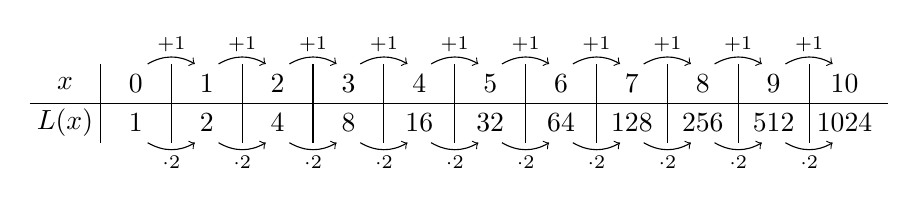
\begin{tikzpicture}
\foreach \i in {0,...,10}{
\draw (\i*0.9,0) -- (\i*0.9,1);
}
\draw (-0.9,0.5) -- (10,0.5);
\foreach \i in {0,...,10}{
\node at (\i*0.9+ 0.45,0.75) {$\i$};
\node at (\i*0.9+0.45,0.25) {$\fpeval{2^{\i}}$};
}
\node at (-0.45,0.75) {$x$};
\node at (-0.45,0.25) {$L(x)$};
\foreach \i in {0,...,9}{
\draw [->] (\i*0.9+0.6,1) to [out=30,in=150] (\i*0.9+1.2,1);
\node at (\i*0.9+0.9,1.25) {$\scriptstyle+1$};
\draw [->] (\i*0.9+0.6,-0) to [out=-30,in=-150] (\i*0.9+1.2,-0);
\node at (\i*0.9+0.9,-0.25) {$\scriptstyle\cdot 2$};
}
\end{tikzpicture}
\caption{De første ti funktionsværdier af $L$, der beskriver antallet af lag af foldet papir.}
\label{fig:sildebenfold}
\end{figure}
På Fig \ref{fig:flagxfold} kan grafen for $L$ ses. 
\begin{figure}[H]
\center
\begin{tikzpicture}
\begin{axis}[axis lines=left,
xlabel = {$x$ (Antal fold)},
ylabel = {$y$ (Antal lag)}]
\addplot[color=blue!40,thick, domain=0:10,samples=1000]{2^x};
\end{axis}
\end{tikzpicture}
\caption{Antal lag af foldet papir som funktion af gentagen foldning}
\label{fig:flagxfold}
\end{figure}
Hvis vi i stedet vil beskrive tykkelsen af det foldede stykke papir, kan vi bruge vores model $L$ fra tidligere. Da et stykke papir er omtrent $0,1$ mm tykt, vil vi kunne beskrive tykkelsen af papiret i cm
\begin{align*}
T(x) = 0.01\cdot L(x) = 0.01\cdot2^x.
\end{align*}
Grafen for $T$ kan ses på Fig. \ref{fig:flagxfold2}. Det ses, at tykkelsen af papiret efter $20$ foldninger er omtrent 10 meter.
\begin{figure}[H]
\center
\begin{tikzpicture}
\begin{axis}[axis lines=left,
xlabel = {$x$ (Antal fold)},
ylabel = {$y$ (Tykkelse i cm)}]
\addplot[color=blue!40,thick, domain=0:20, samples=1000]{0.01*2^x};
\end{axis}
\end{tikzpicture}
\caption{Tykkelse af foldet papir som funktion af gentagen foldning}
\label{fig:flagxfold2}
\end{figure}
\end{exa}
Inspriret af Eksempel \ref{exa:exa1} vil vi se på, hvordan eksponentiel vækst udvikler sig. Vi husker på, at en eksponentialfunktion $f$ kan skrives på formen
\begin{align*}
f(x) = b\cdot a^x,
\end{align*}
for $a,b\in \mathbb{R},a>0$. Ser vi på Fig. \ref{fig:sildebenfold}, så kan vi se, at vi i det tilfælde øger $f(x)$ med en faktor $2$, når vi øger $x$ med 1. Tilsvarende vil vi øge generel eksponentiel vækst med en faktor $a$, når vi øger $x$ med 1. Faktoren $a$ kaldes for fremskrivningsfaktoren. Vi kan se dette fænomen af Fig. \ref{fig:sildegen}
\begin{figure}[H]
\center
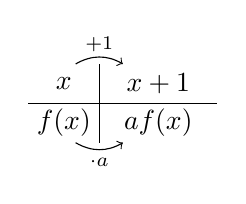
\begin{tikzpicture}
\foreach \i in {0}{
\draw (\i*0.9,0) -- (\i*0.9,1);
}
\draw (-0.9,0.5) -- (1.5,0.5);
\foreach \i in {0}{
\node at (\i*0.9+ 0.75,0.75) {$x+1$};
\node at (\i*0.9+0.75,0.25) {$af(x)$};
}
\node at (-0.45,0.75) {$x$};
\node at (-0.45,0.25) {$f(x)$};
\foreach \i in {0}{
\draw [->] (\i*0.9-0.3,1) to [out=30,in=150] (\i*0.9+0.3,1);
\node at (\i*0.9,1.25) {$\scriptstyle+1$};
\draw [->] (\i*0.9-0.3,-0) to [out=-30,in=-150] (\i*0.9+0.3,-0);
\node at (\i*0.9,-0.25) {$\scriptstyle\cdot a$};
}
\end{tikzpicture}
\caption{Udvikling af eksponentiel vækst.}
\label{fig:sildegen}
\end{figure}
Det er ikke svært at vise, at dette rent faktisk er sandt. Betragter vi
\begin{align*}
f(x+1) = ba^{x+1} = ba^xa = af(x),
\end{align*}
så ses det, at eksponentialfunktioner har en sådan udvikling.
\section*{Opgave 1}
\begin{enumerate}[label=\roman*)]
\item Bevis, at hvis vi øger $x$ med 2 i en eksponentialfunktion $f(x)$, så tilsvarer dette at øge $f(x)$ med en faktor $a^2$. Hvad hvis vi øger $x$ med $3$?
\item Bevis, at hvis vi øger $x$ med $n$ i en eksponentialfunktion $f(x)$, så tilsvarer dette at øge $f(x)$ med en faktor $a^n$.
\end{enumerate}
\section*{Opgave 2}
\begin{enumerate}[label=\roman*)]
\item Hvis vi folder et stykke papir $25$ gange, hvor mange lag papir har vi så? Hvor tykt er dette stykke papir?
\item Hvor mange gange skal vi folde papiret, for at det bliver 1km tykt?
\end{enumerate}
\section*{Opgave 3}
\begin{enumerate}[label=\roman*)]
\item En bakteriekoloni indeholder til tid $t=0$ $B_0 = 100.000$ bakterier. En bakterie deler sig i gennemsnit 1 gang per 4. time, og bakteriekolonien har ubegrænset plads. Beskriv antallet af bakterier som funktion af tiden i timer. Hvor mange bakterier er der i kolonien efter et døgn? Hvornår er der 1 mia. $(10^9)$ bakterier i kolonien?
\item Et glas vand stilles i et rum, og temperaturen i vandet antages at kunne beskrives ved
\begin{align*}
H(t) = 70\cdot(0.97)^t,
\end{align*}
hvor $H(t)$ beskriver temperaturen i grader celcius og $t$ betegner tiden i minutter. Hvor varmt er vandet, når det stilles ind i rummet? Hvor varmt er det efter 5 minutter? Hvor varmt er der i rummet i følge modellen. 
\end{enumerate}

\section*{Opgave 4}
Følgende funktioner er alle eksponentialfunktioner. Vis, hvorfor. Hint: Omskriv dem til formen $f(x) = b\cdot a^x$. 
\begin{align*}
&1) \ f_1(x) = e^{2x}    &&2) \  f_2(x) = 2\cdot 3^x + 4\cdot 3^x  \\
&3) \ f_3(x) =  100000\cdot 2^{\frac{t}{60}}  &&4) \ f_4(x) = 5x^2 +7e^{10x}    \\
\end{align*}

\section*{Opgave 5}
\begin{enumerate}[label=\roman*)]
\item Bevis, at  $\ln(ab) = \ln(a)+\ln(b).$
\item Bevis, at  $\ln(\frac{a}{b}) = \ln(a)-\ln(b)$.
\item Bevis, at  $\ln(a^x) = x\ln(a)$.
\end{enumerate}
Hint: Skriv $a = e^{\ln(a)}$ og $b=e^{\ln(b)}$ og anvend potensregneregler. 
